\documentclass[11pt,a4paper]{article}
\usepackage[utf8]{inputenc}
\usepackage[T1]{fontenc}
\usepackage{lmodern}
\usepackage[spanish,es-tabla]{babel}
\usepackage[margin=2.5cm]{geometry}
\usepackage{amsmath}
\usepackage{graphicx}
\usepackage{booktabs}
\usepackage{siunitx}
\sisetup{output-decimal-marker={,}, group-minimum-digits=5, per-mode=symbol}
\usepackage{enumitem}
\usepackage{hyperref}
\hypersetup{hidelinks}

\title{\textbf{Efecto del grado del imán con entrehierro mínimo impuesto}\\[2pt]
\large\textbf{Conjunto de dos imanes NdFeB D20$\times$4 avellanados, montaje con
separación mínima de \SI{1,5}{mm}}}
\author{}
\date{24 de septiembre de 2026}

\begin{document}
\maketitle

\begin{abstract}
El montaje previsto impone un entrehierro mínimo de \SI{1,5}{mm} entre el conjunto de imanes
y la estructura de acero, por lo que la zona de contacto caracterizada en la memoria anterior
no es accesible. Con la curva ajustada del conjunto actual ---que se comporta como un
\textbf{N35}, $B_r \approx \SI{1,05}{T}$--- como referencia, se evalúa qué se gana al
sustituir los imanes por grados N42 y N52, en dos variantes: cambiando solo el imán, y
agregando un separador que devuelve la fuerza a \SI{1,5}{mm} al valor actual
(\SI{25,6}{N}). El alcance a \SI{2}{N} pasa de \SI{9,85}{mm} a \SI{10,65}{mm} (N42) y
\SI{11,69}{mm} (N52) cambiando solo el imán, a costa de subir la fuerza máxima un
\SI{19}{\percent} y un \SI{47}{\percent}. Si la fuerza máxima debe conservarse, la ganancia
queda en \SI{0,43}{mm} y \SI{0,96}{mm}. \textbf{El grado del imán mueve la cola de la curva
menos de \SI{2}{mm}}: si el objetivo es alcance, la palanca no es el material.
\end{abstract}

\section{Objetivo y alcance}

La memoria de caracterización \emph{Caracterización experimental de la fuerza de atracción de
un par de imanes NdFeB D20$\times$4 avellanados} (7 de septiembre de 2026) dejó registrada la
característica $F(x)$ del conjunto y un modelo de elementos finitos ajustado que la reproduce
con un desvío de \SI{9,3}{\percent}. Aquella memoria concluyó que toda aplicación que dependa
de la fuerza a distancia debe dimensionarse sobre la cola de la curva, nunca sobre el valor de
contacto.

Este informe aplica esa conclusión a la restricción concreta del montaje: un entrehierro
mínimo de \SI{1,5}{mm}. El objetivo es cuantificar si un imán de mayor grado extiende de
forma útil el rango de trabajo, y a qué costo en fuerza máxima.

\section{Planteo}

\subsection{Restricción del montaje}

El montaje no permite acercar el conjunto a menos de \SI{1,5}{mm} del acero. Todo el tramo
$x < \SI{1,5}{mm}$ ---que incluye los \SI{68,7}{N} medidos en contacto--- queda fuera del
rango utilizable. Con los imanes actuales, la fuerza máxima disponible es la de la curva
ajustada en ese punto:
\[
F_\text{máx} = F_{\text{N35}}(\SI{1,5}{mm}) \approx \SI{25,6}{N}.
\]

\subsection{Modelo para otros grados}

Mientras el acero no sature, la fuerza escala con el cuadrado de la remanencia (ecuación~(2)
de la memoria). La curva de cada grado se obtiene escalando la curva ajustada del conjunto
actual por el cociente de remanencias nominales de catálogo:
\begin{equation}
F_g(x) = \left(\frac{B_{r,g}}{B_{r,\text{N35}}}\right)^{\!2} F_{\text{N35}}(x + s),
\label{eq:escala}
\end{equation}
donde $s$ es el espesor de un separador no magnético agregado sobre la cara del imán, que
suma entrehierro a toda la curva. Con $B_{r,\text{N35}} = \SI{1,19}{T}$ y
$B_{r,\text{N42}} = \SI{1,30}{T}$, el factor de fuerza del N42 es $1{,}19$; el del N52 es
$\approx 1{,}48$.

\subsection{Variantes comparadas}

\begin{description}[leftmargin=1.5em, font=\normalfont\bfseries]
  \item[Solo cambiar el imán ($s = 0$).] Toda la curva sube en la proporción del factor de
  fuerza, incluida la fuerza máxima a \SI{1,5}{mm}.
  \item[Imán y separador.] Se elige $s$ de modo que $F_g(\SI{1,5}{mm}) = \SI{25,6}{N}$: la
  fuerza máxima no cambia respecto del conjunto actual y la mejora aparece solo en la cola.
  Resulta $s = \SI{0,37}{mm}$ para el N42 y $s = \SI{0,88}{mm}$ para el N52.
\end{description}

La segunda variante corresponde al caso en que la fuerza máxima está acotada por el resto del
sistema ---por ejemplo, porque el esfuerzo de separación no debe aumentar---; la primera, al
caso en que no lo está.

\section{Resultados}

La figura~\ref{fig:grado} compara las cinco curvas. El panel izquierdo muestra el rango útil
desde \SI{1,5}{mm}, con la zona inaccesible sombreada; el derecho amplía la cola y marca el
entrehierro al que cada variante cae a \SI{2}{N}.

\begin{figure}[htbp]
  \centering
  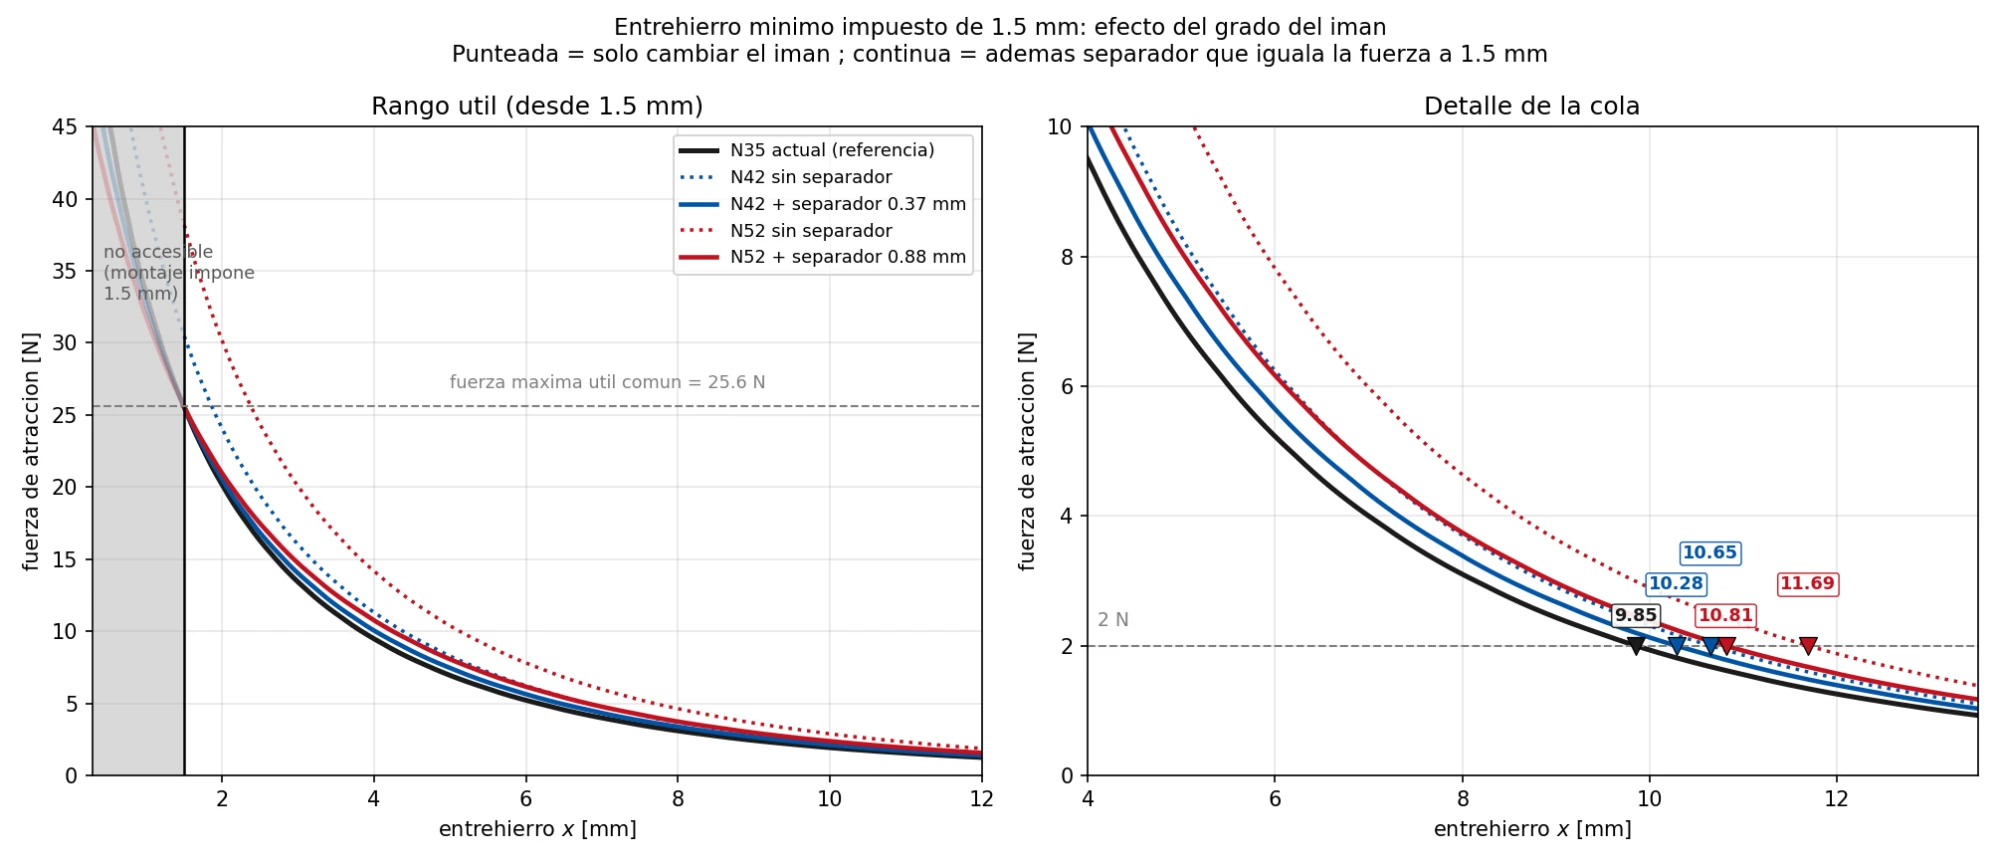
\includegraphics[width=\textwidth]{figuras/grado_entrehierro_1p5.png}
  \caption{Fuerza de atracción con entrehierro mínimo impuesto de \SI{1,5}{mm}. Negro: conjunto
  actual (referencia). Punteadas: solo cambiar el imán. Continuas: imán más separador que
  iguala la fuerza a \SI{1,5}{mm}. Los triángulos del panel derecho marcan el entrehierro al que
  cada curva cae a \SI{2}{N}.}
  \label{fig:grado}
\end{figure}

\begin{table}[htbp]
  \centering
  \caption{Fuerza máxima utilizable y alcance a \SI{2}{N} de cada variante. Las diferencias son
  respecto del conjunto actual.}
  \label{tab:resultados}
  \begin{tabular}{@{}lccccc@{}}
    \toprule
    Variante & Separador & $F(\SI{1,5}{mm})$ & $\Delta F_\text{máx}$ & $x$ a \SI{2}{N} & $\Delta x$ \\
             & [mm]      & [N]               & [\%]                  & [mm]           & [mm] \\
    \midrule
    N35 actual (referencia) & --   & 25,6          & --          & 9,85  & --     \\
    \addlinespace
    N42 sin separador       & --   & $\approx$30,6 & +19         & 10,65 & +0,80  \\
    N42 + separador         & 0,37 & 25,6          & 0           & 10,28 & +0,43  \\
    \addlinespace
    N52 sin separador       & --   & $\approx$38   & $\approx$+47 & 11,69 & +1,84  \\
    N52 + separador         & 0,88 & 25,6          & 0           & 10,81 & +0,96  \\
    \bottomrule
  \end{tabular}
\end{table}

En términos relativos, el alcance a \SI{2}{N} mejora un \SI{8}{\percent} (N42) y un
\SI{19}{\percent} (N52) cambiando solo el imán, y un \SI{4}{\percent} y un \SI{10}{\percent}
si se conserva la fuerza máxima.

\section{Interpretación}

\paragraph{La fuerza crece mucho más que el alcance.}
Pasar de N35 a N52 multiplica toda la curva por $\approx 1{,}48$, pero el punto de \SI{2}{N}
se desplaza solo \SI{1,84}{mm}. Es consecuencia directa del decaimiento de la curva: en la
cola, la fuerza cae aproximadamente a la mitad cada \SIrange{2,5}{3}{mm}, de modo que un factor
constante en la fuerza se traduce en un corrimiento acotado del entrehierro, del orden de
algunas décimas de milímetro por cada \SI{10}{\percent} de fuerza adicional.

\paragraph{El separador consume parte de la ganancia.}
El separador desplaza la curva completa hacia la derecha en $s$, de modo que el alcance a
\SI{2}{N} con separador es, en la aproximación de la ecuación~\eqref{eq:escala}, el alcance
sin separador menos $s$. Como la curva decae más rápido cerca del imán que en la cola, basta un
separador delgado para absorber el aumento de fuerza a \SI{1,5}{mm}, y la mitad de la
ganancia en la cola sobrevive: \SI{0,43}{mm} de \SI{0,80}{mm} en el N42, \SI{0,96}{mm} de
\SI{1,84}{mm} en el N52.

\paragraph{Con separador, las curvas se agrupan en la cola.}
A partir de unos \SI{4}{mm} las variantes con separador quedan dentro de una franja estrecha
alrededor de la referencia (figura~\ref{fig:grado}, panel izquierdo). En la zona donde la
aplicación necesita alcance, el grado del imán es un ajuste fino, no un cambio de régimen.

\paragraph{Consecuencia de diseño.}
Si el requisito es fuerza a distancia, el grado del imán no alcanza para extender el rango de
forma significativa. Las palancas con más efecto sobre la cola son geométricas ---volumen y
altura del imán, retorno de flujo por la cara opuesta, espesor del blanco de acero---, que
este informe no evalúa y deberían estudiarse con el mismo modelo de elementos finitos.

\section{Limitaciones}

\begin{enumerate}
  \item \textbf{Grado real del conjunto actual.} La curva de referencia es la del conjunto
  medido, que \emph{se comporta como} un N35 ($B_r \approx \SI{1,05}{T}$ efectivo). Según la
  sección~6 de la memoria, el grado real puede ser N35 o algo superior. Los factores de la
  ecuación~\eqref{eq:escala} suponen N35 nominal; si el grado real fuera mayor, la ganancia por
  cambiar de imán sería menor que la informada.
  \item \textbf{Pérdidas del ensayo trasladadas.} Escalar la curva medida supone que las
  pérdidas del ensayo ---pintura, espesor finito del blanco, desalineación--- afectan a todos
  los grados en la misma proporción. Es razonable mientras el acero no sature, condición que
  el N52 a \SI{1,5}{mm} exige más que el N35.
  \item \textbf{Remanencias de catálogo.} Se usan valores nominales. Dentro de un mismo grado,
  la dispersión entre fabricantes es de algunos puntos porcentuales en $B_r$, el doble en
  fuerza.
  \item \textbf{Tendencia de los residuos.} La curva de referencia hereda la tendencia
  sistemática de la sección~5.3 de la memoria: en la cola el modelo supera a la medición hasta
  un \SI{20}{\percent}. Los alcances absolutos a \SI{2}{N} pueden estar sobreestimados en unas
  décimas de milímetro; las \emph{diferencias} entre grados, que es lo que este informe
  compara, se ven mucho menos afectadas.
  \item \textbf{Separador ideal.} Se supone no magnético, de espesor uniforme y sin
  compresión. Un separador real agrega tolerancia de espesor al entrehierro.
\end{enumerate}

\section{Conclusiones}

\begin{enumerate}
  \item Con el entrehierro mínimo de \SI{1,5}{mm}, la fuerza máxima utilizable del conjunto
  actual es \SI{25,6}{N}, poco más de un tercio de la fuerza de contacto medida
  (\SI{68,7}{N}).
  \item Cambiar solo el imán sube la fuerza máxima a $\approx\SI{30,6}{N}$ (N42) o
  $\approx\SI{38}{N}$ (N52), y el alcance a \SI{2}{N} a \SI{10,65}{mm} y \SI{11,69}{mm}
  respectivamente.
  \item Si la fuerza máxima debe mantenerse en \SI{25,6}{N}, el separador necesario es de
  \SI{0,37}{mm} (N42) o \SI{0,88}{mm} (N52), y el alcance a \SI{2}{N} mejora solo
  \SI{0,43}{mm} y \SI{0,96}{mm} (tabla~\ref{tab:resultados}).
  \item El grado del imán desplaza la cola de la curva menos de \SI{2}{mm} en el mejor caso.
  No justifica por sí solo el cambio si el objetivo es alcance; sí lo justifica si lo que
  falta es fuerza en el rango cercano y el sistema tolera el aumento.
  \item Para extender el alcance de forma significativa, el próximo paso es evaluar variantes
  geométricas con el modelo de elementos finitos ya validado.
\end{enumerate}

\end{document}
